\chapter{Desenvolvimento}\label{ch:desenvolvimento}

Este capítulo apresenta o desenvolvimento do protótipo de interpretador da linguagem de programação proposta, detalhando as etapas do processo, desde o planejamento até a implementação.

O desenvolvimento do protótipo tem como objetivo, com base na seção \ref{sec:obj_geral}, provar a viabilidade inicial da implementação do \textit{design} da linguagem, além de fornecer uma base para futuras pesquisas e aprimoramentos. Assim como descrito no capítulo \ref{ch:metodologia}, o desenvolvimento foi dividido nas etapas de planejamento e implementação de modo a separar as responsabilidades do desenvolvimento.

\section{Visão Geral da Solução}

Usando como base os critérios e características do \textit{design} de linguagens de programação descritos na seção \ref{sec:design_linguagem}, o planejamento da solução foi dado pela definição de alto nível da sintaxe e semântica da linguagem, além da escolha das tecnologias a serem utilizadas na implementação do protótipo.

Já na implementação, o foco foi a construção do interpretador da linguagem proposta no planejamento, iniciando pela criação dos analisadores léxico e sintático, seguidos pelo analisador semântico e, por fim, a implementação do interpretador propriamente dito. Como base para a implementação, foi principalmente utilizado o livro \textit{Crafting Interpreters} \cite{craftinginterpreters}, além de artigos sobre ECS escritos por Sander Mertens e documentação de bibliotecas de ECS, como Flecs \cite{flecs} e Bevy \cite{bevy}.

De modo a permitir uma visão ampla sobre a implementação e a conexão entre suas partes, a \autoref{fig:diagrama_geral} apresenta o diagrama geral do protótipo de interpretador proposto pelo trabalho. Nele, nota-se a divisão entre as diferentes fases do interpretador e como elas se conectam em um fluxo linear de dados, desde a geração dos \textit{tokens} até a ampliação da AST.

\begin{figure}[H]
	\centering
	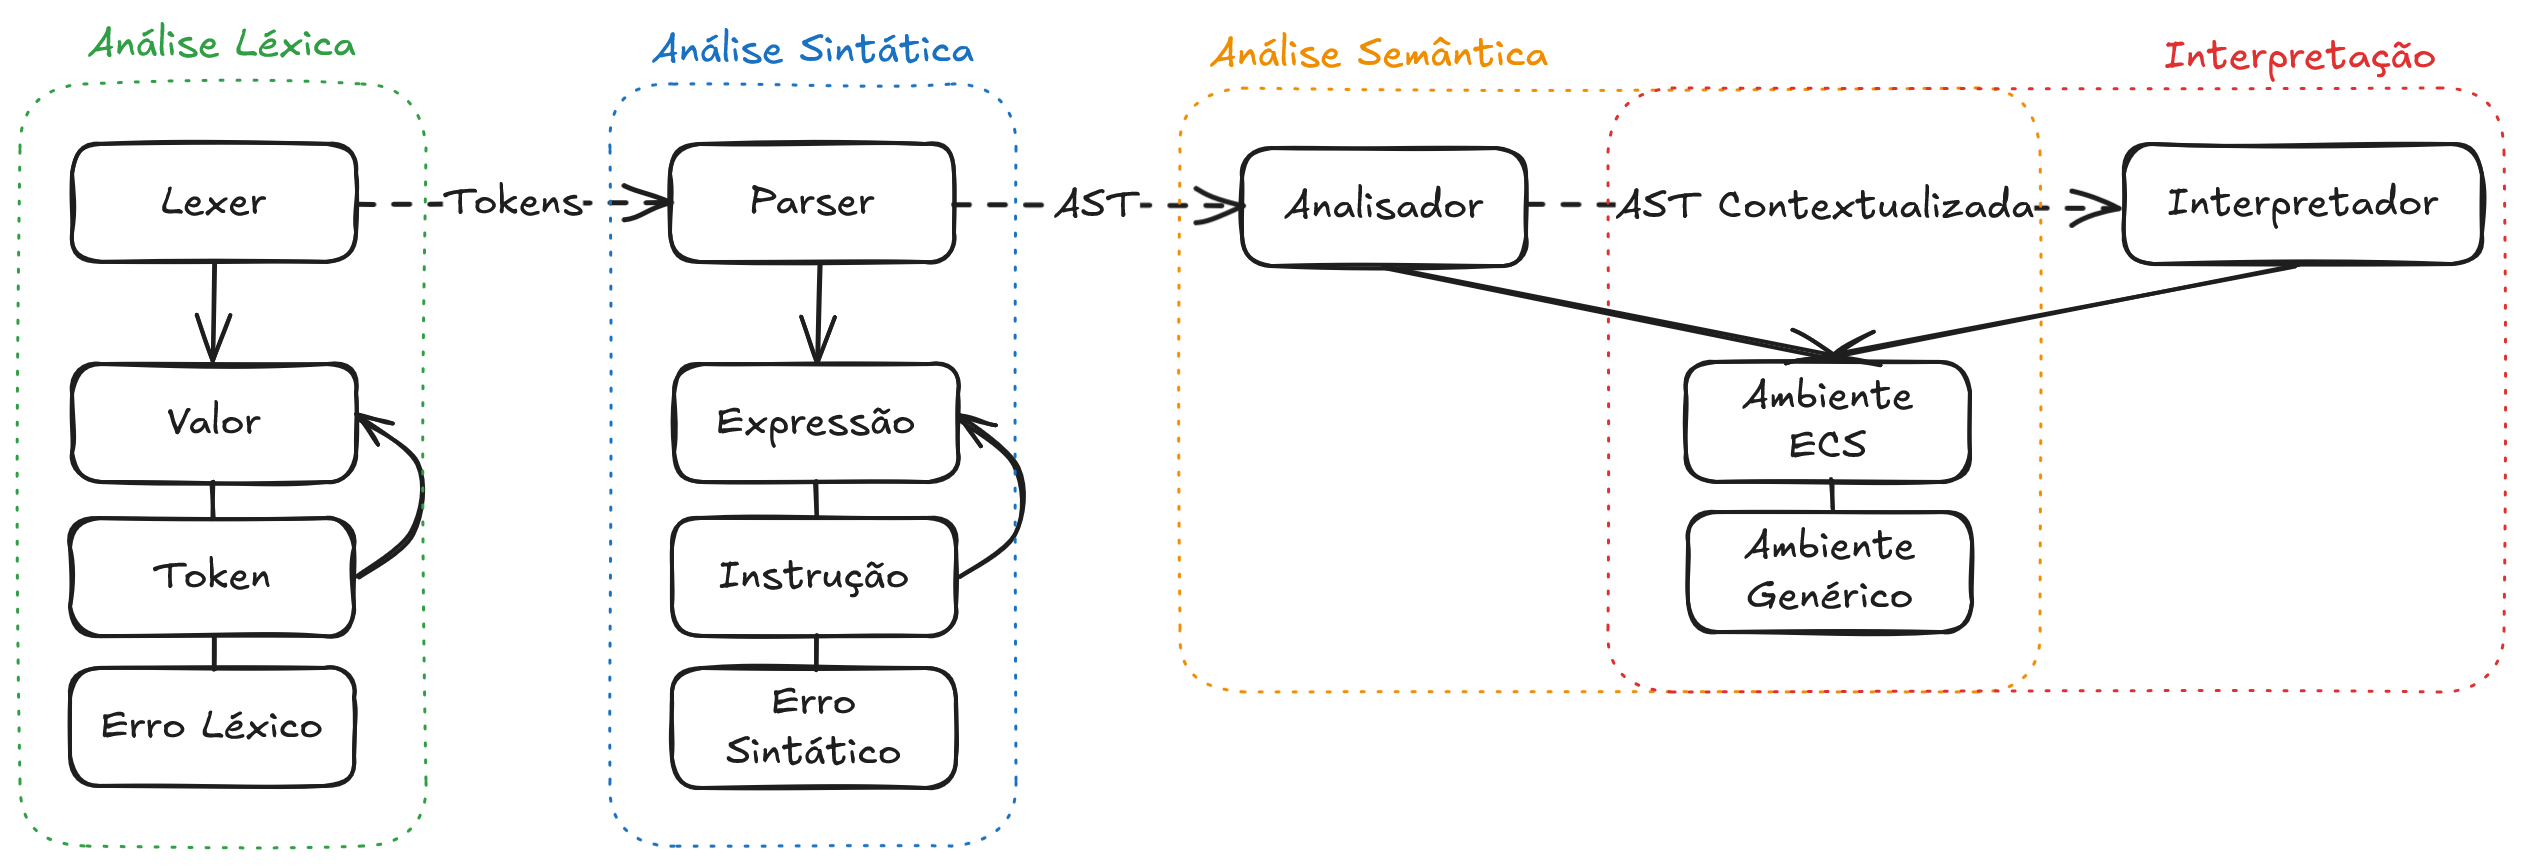
\includegraphics[width=0.65\textheight]{diagrama_geral.excalidraw.png}
	\caption{Diagrama geral do protótipo de interpretador.}
	\fonte{Elaboração própria.}
	\label{fig:diagrama_geral}
\end{figure}

De forma mais detalhada, nota-se como cada fase depende de outros componentes para funcionar, como o \textit{lexer}, que depende da definição de \textit{token}. Cada componente está agrupado com a fase que o produz, como as definições de expressão e instrução, que estão agrupadas com o \textit{parser}, que as produz.

Até então, pode-se notar como foram utilizados termos como \textit{lexer} e \textit{parser} ao invés de analisador léxico e analisador sintático, respectivamente. Isso se deve ao fato de que, a partir deste ponto, esses serão os termos utilizados para se referir mais especificamente aos componentes do interpretador, enquanto os termos em português serão utilizados para se referir às fases que caracterizam estes componentes. A \autoref{tab:terminologia_fases} ilustra a diferença de uso entre os termos.

\begin{table}[h]
	\centering
	\caption{Terminologia utilizada para se referir às fases do interpretador e seus componentes.}
	{
		\begin{tabular}{ll}
			\hline
			\textbf{Fase}          & \textbf{Componente} \\ \hline
			Análise Léxica      & \textit{Lexer}      \\
			Análise Sintática   & \textit{Parser}     \\
			Análise Semântica   & \textit{Analyzer}                   \\
			Interpretação       & \textit{Interpreter}                   \\ \hline
		\end{tabular}
	}
	\fonte{Elaboração própria com base na terminologia usada em \citeonline{craftinginterpreters}.}
	\label{tab:terminologia_fases}
\end{table}
